\documentclass[11pt]{article}

% basic packages
\usepackage[margin=1in]{geometry}
\usepackage[pdftex]{graphicx}
\usepackage{amsmath,amssymb,amsthm}
\usepackage{william}

% page formatting
\usepackage{fancyhdr}
\pagestyle{fancy}

\renewcommand{\sectionmark}[1]{\markright{\textsf{\arabic{section}. #1}}}
\renewcommand{\subsectionmark}[1]{}
\lhead{\textbf{\thepage} \ \ \nouppercase{\rightmark}}
\chead{}
\rhead{}
\lfoot{}
\cfoot{}
\rfoot{}
\setlength{\headheight}{14pt}

\linespread{1.03}
\setlength{\parindent}{0.2in}
\setcounter{secnumdepth}{2}
\setcounter{tocdepth}{2}

\newcommand{\supp}{\operatorname{supp}}

\begin{document}

\thispagestyle{empty}
\bigskip \
\vspace{0.1cm}

\begin{center}
{\fontsize{22}{22} \selectfont My Answers to}
\vskip 16pt
{\fontsize{36}{36} \selectfont \bf \sffamily Random Questions I Think About}
\vskip 24pt
{\fontsize{18}{18} \selectfont \rmfamily \href{https://will-lancer.github.io}{Will Lancer}}
\vskip 6pt
{\fontsize{14}{14} \selectfont \ttfamily will.m.lancer@gmail.com}
\vskip 24pt
\end{center}

{\parindent0pt \baselineskip=15.5pt}
\noin
Write-ups of random questions I've thought about and tried to understand
more deeply. Started doing this at the end of May 2026. In the age of LLMs,
there is no excuse for not understanding anything that you work with as deeply
as you'd like.

I'll note that most questions that I ask here are very basic, as that's how I tend
to operate. Unless I understand something in its most natural setting, I am confused.
Asking basic questions is largely how I get unconfused.

\newpage
\microtoc
\newpage

\section{Basic physics}

\subsection{Statistical mechanics}

\subsubsection{What is an ensemble?}

\note{to-do}

\subsubsection{Why do physical systems minimize their free energy?}


We'll show this using the saddle-point argument. Consider a partition function,
\begin{align*}
Z(\beta) & = \int dE\, \rho(E)\, e^{-\beta E} = \int dE\, e^{S(E) - \beta E}.
\end{align*}
If the system is large ($N \sim 10^{23}$), it is well-approximated 
by its saddle-point value if $S$ and $E$ are extensive quantities,
\begin{align*}
Z(\beta) & \approx e^{\max(S(E) - \beta E)}.
\end{align*}
\note{need to completely justify this claim}
Looking more closely at the quantity in parentheses gives
\begin{align*}
    \max(S(E) - \beta E) \iff \min(\beta E - S) \iff \min(E - TS) \eqqcolon \min{F}.
\end{align*}
So, it's overwhelmingly likely\footnote{The probability that a system takes a
non-equilibrium free energy value is on the order of $e^{-10^{23}}$. This is
comically tiny.} that a system will take a value that 
minimizes its free-energy, $F \coloneqq E - TS$.

Notice that the two assumptions in this model beget some of its failure modes:
we assumed that $N \sim 10^{23}$ and that $E$ and $S$ were extensive quantities
in $N$. \note{exampels of where this doesn't hold}

\qed

\subsubsection{What is the chemical potential?}

\note{to-do}

\newpage

\section{Basic math}

\subsection{Analysis}

\subsubsection{Big-O notation}

\note{finish}

\subsubsection{Useful fact about Fourier transforms: the uncertainty principle}

Statement from Hannah Cairo: (see the talk \href{https://youtu.be/3ZeH_8sTyKA?si=NR79zGW6PTfWMNHs}{here})
\begin{iidea}
    [The uncertainty principle]
    If a function $f$ has support on an interval $[-R, R]$, then its Fourier transform
    $\widetilde{f}$ is essentially constant on $[-1/R, 1/R]$.
\end{iidea}
This generalizes to boxes \note{is essentially a special word here? i'd prefer
to use approximately}
\begin{iidea}
    If $\supp{f} \subset [-A, A] \times [-B, B] \times [-C, C]$, then $\widetilde{f}$
    is essentially constant on boxes of $[-1/A, 1/A] \times [-1/B, 1/B] \times [-1/C, 1/C]$.
\end{iidea}
We can easily draw this idea to get some intuition for the result:
\begin{figure}[H]
    \centering
    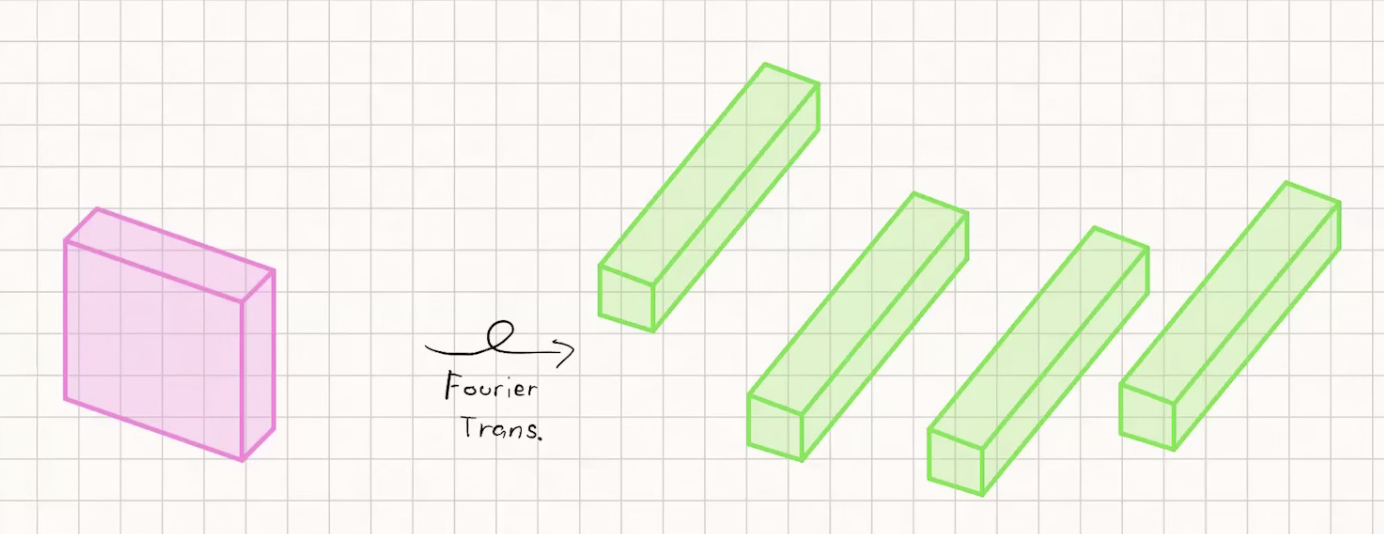
\includegraphics[width=0.8\textwidth]{figures/cairo_pic.png}
    \caption{Support of $f$ on the left, and \note{support ?} of Fourier transform
    on the right.}
\end{figure}

Notice the duality between small $R$ and big $k \sim 1/R$, and vice-versa---this
is reflected in the dimensions of the boxes on the left and right-hand side above.
The reason why there are multiple boxes is because \note{not sure honestly.
how does the support of a function fourier transform? this is a useful question
to answer for physical considerations as well! i.e. $f(x)$ has some supp, wb 
$\widetilde{f}(k)$?}


% This is an instantiation of the uncertainty principle,
% \begin{align*}
%     \Delta x \, \Delta k \gtrsim 1.
% \end{align*}

% \note{understand the above. why isn't it equal. also what is $\Delta$?}

% \note{include pictoral notation! This is interesting}

\newpage

\section{Physics topics}

\subsection{Condensed matter}

\subsubsection{What is a Fermi surface?}

We'll start with an example. Take a fermionic gas in a cube with side length $L$.
Its possible energies are
\begin{align*}
    E_\bfk = \frac{\hbar^2 \bfk^2}{2m} = \frac{\hbar^2 \mathbf{n}^2}{2mL^2}. 
\end{align*}
Since these particles are fermions, they obey the Pauli exclusion principle.
Thus, if we fill the states starting from the ground state upwards, we
\note{nope. don't understand why $\mu$ even exists or is a thing}

\subsection{Quantum field theory}


\end{document}